\documentclass[prb,preprint]{revtex4-1}
\usepackage{graphicx}
\usepackage{amsmath}

\begin{document}

\title{Computer-controlled sinusoidal drive mechanism}

\author{Eric Ayars}
\affiliation{California State University Chico}
\email{eayars@csuchico.edu}
\author{Nicholas Nelson}
\affiliation{California State University Chico}

\date{\today}

%Editor�s Note: This paper presents the design for a relatively simple and very affordable sinusoidal driver controlled by a microcontroller. Given the importance of driven oscillations and resonance throughout physics, the device is useful for classroom demonstrations and instructional laboratories in introductory as well as upper-level courses. The limitations of commercial drivers is explained, while a mathematical derivation presents how this device overcomes those limitations. Details of the construction of the device are available on github.


\begin{abstract}
We describe an inexpensive computer-controlled sinusoidal drive mechanism for dynamics carts (and other applications) with applications for resonance, normal-modes, and chaos experiments.
The driver arm moves in a non-sinusoidal motion such that the cosine error inherent to its design \emph{corrects} the motion, making the output a more nearly single-frequency wave than commercially available drivers.
In addition, the design facilitates easy access to the drive position at any point in time, allowing for the collection of phase information and synchronization of data to drive position.
\end{abstract}

\maketitle

\section{Introduction}

Dynamics carts and tracks are in such common use in introductory physics courses that a list of applications is unnecessary for readers of this journal.
They are less commonly used in the advanced undergraduate mechanics course, however.
Recently, one of the authors wanted to use dynamics carts in their upper-division mechanics course to show resonance response curves and normal modes, and needed a robust sinusoidal drive mechanism.

\section{Existing solutions}
There are several commercial options available for this need; none of them are ideal. 
One option is a \emph{speaker-type driver}, such as the Vernier Power Amplifier Accessory Speaker.\cite{VernierSpeaker}  
This type of driver uses an AC signal to a long-throw bass speaker coil and magnet to drive oscillations. 
The frequency can be precisely controlled using the function generator providing the AC signal, but the amplitude of oscillation depends on the load, and the position of the driver is only approximately sinusoidal at low amplitudes and high frequencies.
There are significant higher harmonics in the driver motion that can cause experimental artifacts, particularly in sensitive resonance and chaos experiments.
Depending on the function generator used, a trigger signal may be available to synchronize data acquisition, but at most once per period, so driver position is not precisely known.

Another commercially available option is the \emph{circular driver}, such as the PASCO ME-8750.\cite{PascoMotor} 
This type of driver uses a geared DC motor with an arm attaching a string at some radius $R$ from the axis. 
%[**The quantity L is never explicitly defined. Please add definition soemwhere above next sentence. One suggestion is below.**]
The string then goes through a guide, 
%[**Added definition here.**]
%perfect, thanks. -ea
where $L$ is the distance of the guide from the center of rotation,
converting the angular position $\theta$ of the motor to linear position $x$. (See Fig.~\ref{fig:circular}, which also shows various parameters for later calculations.) 
%[**Below, this inequality is always written as R<<L. Consider changing for consistency, as given below.**] 
%For $L\gg R$,
%Agreed.-ea
 For $R \ll L$, $x$ is approximately sinusoidal. 
The amplitude of the motion for this driver is independent of load, and the frequency can be adjusted by changing the speed the motor.
There are multiple limitations in the circular driver: it's impossible to adjust the amplitude on the fly, accurate position information is not available, precise frequency control is difficult, and $x$ is only approximately sinusoidal when $R \ll L$.
The requirement that $R \ll L$ puts inconvenient constraints on either the maximum amplitude or the overall length of the apparatus, and the 
%[**Cosine error is not defined. Please consider adding definition as below (I'm not positive I have correct definition.**]
``cosine error'' %(due to misalignment of the rotation plane with the $x$-direction)
% This is a tricky one\dots Does the below work for you? -ea
(due to the misalignment between the motion of the attachment point and the direction of $\ell$)
%[**The following statement is a bit unclear. A suggested change for clarity is below.**]
%for $R$ not $\ll L$ 
when the condition $R \ll L$ is not met introduces significant frequency components at multiples of the drive frequency. 
As with the 
% below, changed ``speaker'' type drier,
speaker-type driver, these frequency components can cause measurement artifacts.

%[**The spring appears to be attached to a circular wheel instead of a rotating arm. Please consider redrawing for clarity.**]
% redrawn -ea
\begin{figure}[ht]
	\begin{center}
		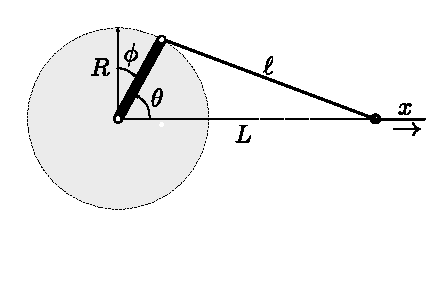
\includegraphics[width=4in]{geometry_2}
	\end{center}
	\caption{Geometric layout, and variables, for both the circular driver and this servo-controlled driver.
%[**Added definitions.**]
	$\ell$ is instantaneous length of string from rotating arm to guide (indicated by small circle).	
	}
	\label{fig:circular}
\end{figure}

\section{Our approach}
We decided to use geometry identical to that of the circular driver in Fig.~\ref{fig:circular}, but with a servomotor from a radio-control car steering system providing an oscillatory motion, instead of driving the motion in a full circle at a constant angular velocity. 
Controlling a servo is very easy with a microcontroller: we chose a Teensy 4.0 for its combination of low price, high speed, breadboard-friendly form factor, and floating-point math capability.
Using an oscillating servomotor output allows complete on-the-fly control of both frequency and amplitude, as well as precise static positioning, when desired. 

The only disadvantage remaining in this approach is the existence of harmonics arising from the cosine error inherent to this geometry. 
Normally, if one is driving a sinusoidal output with a microcontroller, the
%[**Better word choice??**]
% way to do it
standard procedure
 is to generate a look-up table (LUT) of output values in the microcontroller memory.
The microcontroller looks up a value in the array, 
%sets its output 
Sets the output
%[**add "voltage"??**]
%voltage
% Not necessarily voltage. In this case it's position. How about 'sets THE output to that value', since the units of the output can be \dots whatever is oscillating!
to that value, waits some time interval $\Delta t$, then looks up the next value and repeats the process. 
The frequency of the output waveform depends on the timestep $\Delta t$ between LUT values.
For a sinusoidal output, the look-up table would consist of values of sine (or cosine) evenly distributed over a complete period $T$.
%But
%[**Suggested change below**]
However, in our case,
 we don't want the servo motion $\phi$ to be sinusoidal, we want $x$ to be sinusoidal! That is,
\begin{equation}\label{x}
	x = A \sin(\omega t) 
\end{equation}
%This is equivalent to saying that
%[**A suggested change for clarity**] Good -ea
From Fig.~\ref{fig:circular}, we see that Eq.~(\ref{x}) implies that the instantaneous length of the string from the rotating arm to the guide is given by
\begin{equation} \label{l_desired}
	\ell(t) = \ell_o + A \sin(\omega t)
\end{equation}
where 
\begin{equation}
	\ell_o \equiv \sqrt{R^2+L^2}
\end{equation}
%[**The meaning of this phrase is unclear. Please consider re-writing for clarity.**]
%The servo is centered at $\phi=0$, 
The servo angular position oscillates around $\phi=0$, 
and we want to find $\phi(t)$ such that $\ell(t)$ has the desired solution.
%[**Suggested change for clarity below.**]
%Start with the law of cosines:
%\begin{eqnarray} 
%	\ell^2 &=& R^2 + L^2 - 2 R L \cos\theta\\
%		&=& R^2 + L^2 - 2 R L \sin\phi\\
%	\ell &=& \left[ R^2+L^2 - r R L \sin\phi \right]^{\frac{1}{2}} = \sqrt{R^2+L^2} + A \sin(\omega t)
%\end{eqnarray}
Start with the law of cosines:
\begin{eqnarray} 
	\ell^2 &=& R^2 + L^2 - 2 R L \cos\theta\\
		&=& R^2 + L^2 - 2 R L \sin\phi \label{l_derived}
\end{eqnarray}
Then, setting Eq.~(\ref{l_derived}) equal to Eq.~(\ref{l_desired}), we get
\begin{equation}
\ell = \left[ R^2+L^2 - r R L \sin\phi \right]^{\frac{1}{2}} = \sqrt{R^2+L^2} + A \sin(\omega t)
\end{equation}
% Yes, that's an improvement. Thanks. -ea

A few more careful steps of algebra give us an equation for the desired motion of the servo:
\begin{equation} \label{eq:phi}
	\phi(t) = \sin^{-1} \left[\frac{1}{2RL}\left(2\ell_o A\sin(\omega t) + A^2 \sin^2(\omega t)\right)\right]
\end{equation}

Equation~(\ref{eq:phi}) is not particularly user-friendly, but one can check it for special cases. 
By geometric necessity, $A<R$, so if $R\ll L$ then $\ell_o \approx L$, $\phi$ is small, and 
\begin{equation}
	\phi(t) \approx \frac{A}{R}\sin(\omega t)
\end{equation}
as one would expect for this limiting-case geometry.
When $R$ is not small compared to $L$, one can consider the limiting case of $A \ll R$. 
In this case, the first term dominates and $\phi(t) \propto \sin(\omega t)$ as one would intuitively expect. 

For the general case, though, the microcontroller can move the servo through the curve described by Eq.~(\ref{eq:phi}) just as easily as through a sine curve. 
Instead of building a LUT containing values of $A\sin(\omega t)$ at each time $t$, the microcontroller needs to build the LUT with values of $\phi(t)$.
The values of $\phi$ depend on $A$, so the LUT must be recalculated each time the amplitude is adjusted. 
The Teensy microcontroller can recalculate this array of 256 LUT values in a few hundred microseconds, a negligible delay which in any case occurs only on amplitude changes.

%[**A circuit diagram would be very helpful here. It may be in the github material, but I couldn't find it.**]
% I think we should leave it in the github materials. I had omitted it earlier, it's there now. Take a look and see what you think: it's literally just one pin from the microcontroller and a power connection.
% File Drive/Circuit.pdf on the Github site.
% But if you want it here, we can put it here.
\begin{figure}[ht]
	\begin{center}
		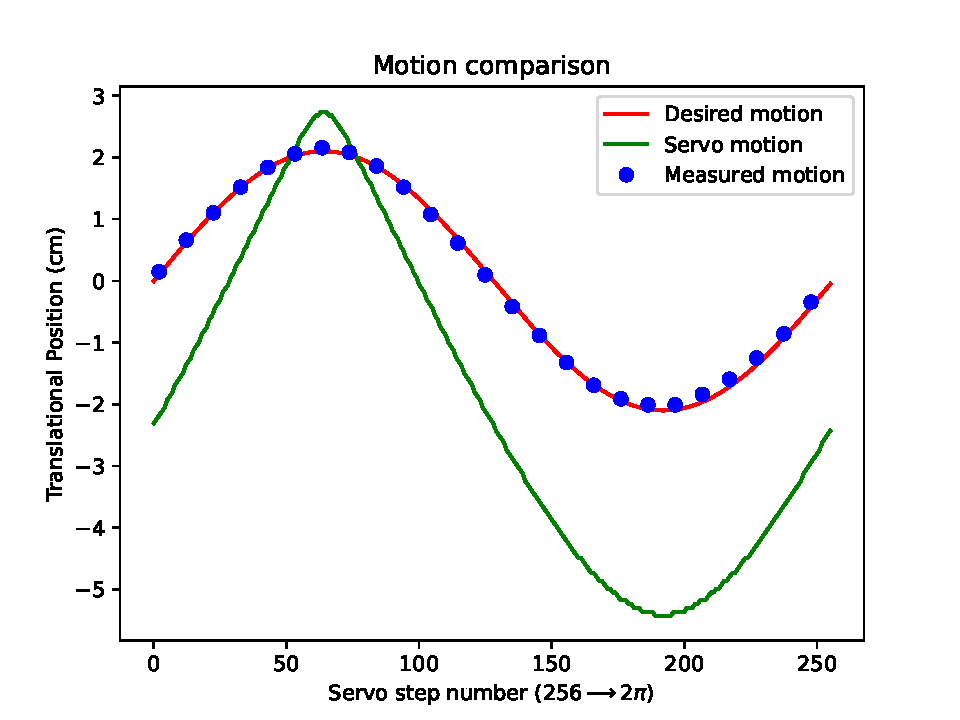
\includegraphics[width=5in]{comparison}
	\end{center}
	\caption{A plot of the servo motion $\phi$, as well as the resulting sinusoidal motion in $x$.}
	\label{fig:motion}
\end{figure}

\begin{figure}[ht]
	\begin{center}
		\includegraphics[width=5in]{device}
	\end{center}
	\caption{A photo of the completed device, showing the circuitboard, servo (EcoPower WP110T), and routing of the drive string.}
	\label{fig:device}
\end{figure}

Figure \ref{fig:motion} shows the non-sinusoidal motion of the servo end ($R\phi$) and the resulting sinusoidal motion of the output $x$, as measured by a Vernier GoDirect Sensor Cart.\cite{VernierCart}

The final construction step was to design a simple 3D-printed mount to hold the servo and the microcontroller board in place at one end of the dynamics track, as shown in Fig.~\ref{fig:device}.
For the fairly compact driver head we made, the improvement in the motion at maximum amplitude was an approximately 20 dB decrease in the first harmonic compared to sinusoidal $\phi$.

%[**Suggested alternate wording for this sentence below.**] An improvement, thanks. -ea
%There are several advantages to having a microcontroller-based mechanical driver such as this. 
Our microcontroller-based mechanical driver has several advantages in comparison to the commercially available drivers mentioned previously. 
A microcontroller can do much more than merely drive a given constant frequency and amplitude. 
The firmware we wrote for the microcontroller includes SCPI communications capability, so the device can be easily interfaced to LabVIEW, Python, or any other serial-capable programming language through the USB port on the Teensy 4.0 board.
For the purpose of the mechanics course demonstration that sparked this project, a simple Python program to control frequency and amplitude sufficed to do what was needed. Other programs can be easily created to sweep through a range of frequencies for resonance curve analysis, or a range of amplitudes for investigations of chaotic oscillators, e.g., see Fig.~\ref{fig:2-carts}.
\begin{figure}[h]
	\begin{center}
		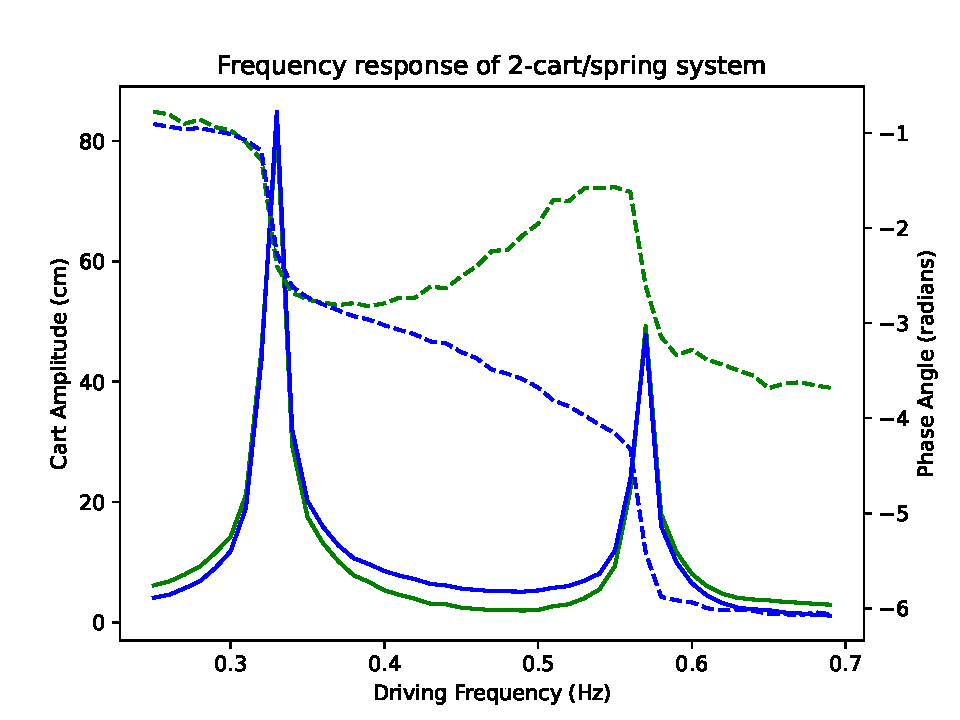
\includegraphics{2-cart_response}
	\end{center}
	\caption{Amplitude and phase response for two Vernier GoDirect Carts connected by springs, showing the normal mode resonances as well as the corresponding phase differences between the carts and the driver.}
	\label{fig:2-carts}
\end{figure}
In addition, it should be noted that since the microcontroller is generating the output waveform stepwise with a LUT, it is trivial to obtain exact position data for the driver at any point in time. 
This allows for the collection of phase information for the driver, which is not available with the commercially available options described here. 
(Note the phase information in Fig.~\ref{fig:2-carts}.)
It also allows for the synchronization of data to drive position, so that if, for example, one were using our device to drive a chaotic oscillator, one could collect data to generate a full set of Poincar\'e sections.

\section{Additional Applications}
Although the purpose of this design is to generate a sinusoidal motion, the device is not limited to sinusoidal motion.
By calculating appropriate LUT values, the microcontroller can drive any arbitrary motion of the servo arm, within the limits set by the servo speed. 
Applications that could be of particular interest in labs beyond the first year include multi-frequency drive output for investigations of mode-locking and other nonlinear phenomena, or driving with beats for investigations of energy transfer between modes.
Modifications to the circuit and firmware could allow for experimental feedback so that the drive frequency or amplitude is adjusted in real time based on the response of the system being driven.
This could be used for investigations of control theory and similar applications.

\section{Limitations}
The main limitation to our driver design is the maximum frequency available. 
Due to the response time of the servo, the maximum frequency is around 3--5 Hz, depending on the amplitude of motion.
This range of frequencies works well for apparatus such as carts and Duffing oscillators and other mechanical systems, but if higher frequencies are necessary the speaker-type driver may be a better choice, despite its harmonic limitations.

Another limitation is that the output becomes noticeably `stepped' at low amplitudes.
The servo is controlled by a pulse-width modulation (PWM) signal, and the resolution of the PWM signal is finite.
At low amplitudes, the change in $\phi$ between adjacent LUT values becomes smaller than the resolution of the PWM signal, so the servo cannot be moved to the desired position and instead jumps to one of the two closest positions it can achieve. 
If low amplitudes are desired, it is best to use a smaller servo arm (smaller value of $R$) to increase the required change in $\phi$ for a given change in $x$, but then that limits the maximum amplitude. 

\section{Conclusions}
%[**The meaning of the following sentence is unclear. Please consider re-writing for clarity.**]
%By using a microcontroller to move a servo arm in a geometry for which there is cosine error, we can use the microcontroller to generate a specific non-sinusoidal motion which the cosine error then corrects to make the motion sinusoidal.
This geometry has an inherent cosine error. 
By using a microcontroller to control the position of the servo, we can generate a specific non-sinusoidal \emph{servo} motion which the cosine error corrects to make the \emph{drive} motion sinusoidal.
The microcontroller also provides computer control of frequency, amplitude, and (if desired) static position of the driver and allows easy control of the device via Python, LabVIEW, and other programming languages. 
The device allows for time-synchronized position data, which opens up numerous possibilities for experiments beyond the introductory course.

\section{Want to build one?}
Microcontroller firmware, example Python control code, and 3D print files for this device are available on GitHub at \url{https://github.com/EricAyars/Cart-driver}

The Authors have no conflicts of interest to disclose.

\begin{thebibliography}{3}
\bibitem{VernierSpeaker} Vernier Science Education ``Power Amplifier Accessory Speaker''' \url{<https://www.vernier.com/product/power-amplifier-accessory-speaker/>}

\bibitem{PascoMotor} PASCO Scientific ``Mechanical Oscillator Driver''' \url{<https://www.pasco.com/products/lab-apparatus/mechanics/dynamics-accessories/mechanical-oscillator-driver>}

\bibitem{VernierCart} Vernier Science Education ``GoDirect Sensor Cart'' \url{<https://www.vernier.com/product/go-direct-sensor-cart/>}

\end{thebibliography}

\end{document}

